\documentclass[spanish,12pt,a4paper,titlepage]{report}
\usepackage[utf8]{inputenc}
\usepackage{graphicx}
\usepackage{subfig}
\usepackage{float}
\usepackage{wrapfig}
\usepackage{multirow}
\usepackage{caption}
\usepackage[spanish]{babel}
\usepackage[dvips]{hyperref}
\usepackage{amssymb}
\usepackage{listings}
\usepackage{epsfig}
\usepackage{amsmath}
\usepackage{array}
\usepackage[table]{xcolor}
\usepackage{multirow}
%\usepackage[Sonny]{fncychap}
\usepackage[Lenny]{fncychap}
%\usepackage[Glenn]{fncychap}
%\usepackage[Conny]{fncychap}
%\usepackage[Rejne]{fncychap}
%\usepackage[Bjarne]{fncychap}
%\usepackage[Bjornstrup]{fncychap}

%\usepackage{subfiles}
%\usepackage{framed}

\setlength{\topmargin}{-1.5cm}
\setlength{\textheight}{25cm}
\setlength{\oddsidemargin}{0.3cm} 
\setlength{\textwidth}{15cm}
\setlength{\columnsep}{0cm}


\newcommand{\grad}{\hspace{-2mm}$\phantom{a}^{\circ}$}
\newcommand{\degc}{$^\circ$C}
\begin{document}


\chapter{Magnetómetro}
\label{chap:magnetometro}

\section{Objetivos}

El objetivo de estas pruebas es comprender y caracterizar el magnetómetro de 3 ejes Honeywell HMC5583, incorporado para asistir en la determinación de la orientación absoluta del cuadricóptero.

\section{Materiales}
\label{sec:materiales}

\begin{itemize}
\item Mesa de madera de 1.5m de largo.
\item Laptop.
\item Hilo y clavos.
\item Mesa nivelable.
\item Cubo de lapacho
\item IMU ``Mongoose'' de CKDevices, con un HMC5583.
\item Foto satelital, con información sobre coordenadas.
\item Mesa nivelable, con una superficie que se pueda inclinar en ángulos conocidos.
\item Escuadra
\end{itemize}

\newpage

\section{Procedimiento}
\label{sec:procedimiento}

El modelo adoptado para relacionar las medidas de campo magnético sin calibrar con las medidas calibradas es idéntico al utilizado a la hora de calibrar el acelerómetro y el giróscopo, el procedimiento utilizado es el descrito por \ref{bib:Merayo}. Se toma una serie de medidas de campo magnético terrestre en diversas orientaciones. Para asegurar la calidad de los datos es recomendable tomar medidas distribuidas uniformemente en todas las direcciones. Dado que el campo es constante, la gráfica de las medidas anteriores debería resultar en una esfera con centro en el origen de radio igual al módulo del campo magnético de la Tierra. Al no tener un sensor calibrado el resultado será un elipsoide. Se utilizó un algoritmo desarrollado por \emph{Alain Barraud} para realizar la calibración, dicho algoritmo no es otra cosa que la implementación de la minimización presente en el método propuesto.\\

Una vez calibrado el sensor se procede a verificar la exactitud que ofrece el mismo para determinar la orientación de la plataforma. Con dicho objetivo se ubica la plataforma alineada en una dirección conocida, sobre una mesa nivelada (de forma que se encuentre paralela a la superficie de la Tierra). Se toman las medidas del campo magnético para distintas orientaciones.\\
Cabe aclarar que el Norte magn\'etico no se corresponde con el Norte geogr\'afico en toda la Tierra, sino que por el contrario (dependiendo de la regi\'on del mundo) presenta una declinaci\'on. Es decir que tenemos una componente del campo magn\'etico en la dirección Oeste-Este adem\'as de la componente Sur-Norte. La declinaci\'on es diferente en cada punto de la 
Tierra. En particular en Uruguay la misma es de $-9.74^{\circ}$ seg\'un la convenci\'on mundial, es decir que el Norte magn\'etico se encuentra $9.74^{\circ}$ al Oeste del Norte geogr\'afico. 

\section{Resultados y Análisis}
En la figura \ref{fig:bola} se observan graficadas las medidas de campo magnético con el sensor descalibrado en los ejes solidarios a la plataforma. Como era de esperarse en la medida con el sensor descalibrado no se obtiene una esfera, esto se debe a que las ganancias en cada eje no son las adecuadas. Por otra parte los ejes principales tampoco son colineales con $X_q, Y_q $ y $ Z_q$. Debido a los \emph{offset} en cada dirección el centro del elipsoide no concuerda con el origen. En la figura \ref{fig:bolacalib} tenemos las medidas de campo magnético con el sensor calibrado. En primer lugar es interesante destacar que se tiene una esfera centrada en el origen, por lo tanto la calibración puede calificarse de exitosa. La magnitud que medimos luego del proceso de calibración se encuentra normalizada. Dado que utilizaremos dicho sensor para determinar una orientación, nos interesan simplemente las relaciones entre las componentes medidas en cada eje del sensor, por lo tanto trabajar con las medidas normalizadas arroja el mismo resultado que trabajar con las medidas de campo en Teslas o Gauss.


\begin{figure}
  \begin{center}
	\subfloat[Con el sensor descalibrado]{\label{fig:bola}
	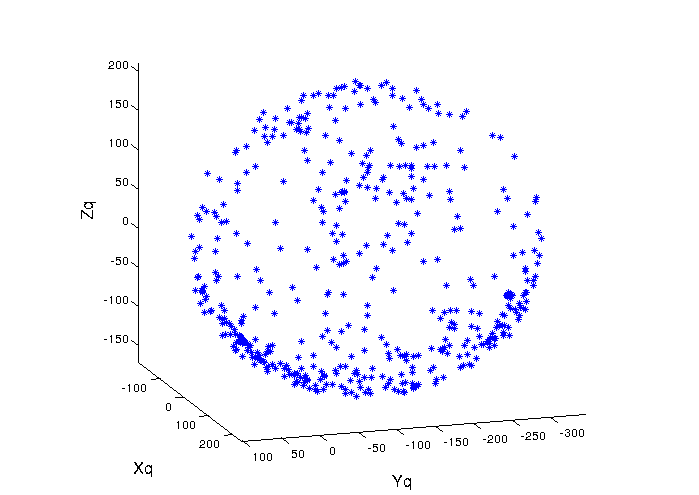
\includegraphics[width=0.5\textwidth]
		{./pics/bola.png}}
	\subfloat[Con el sensor calibrado]{\label{fig:bolacalib}
	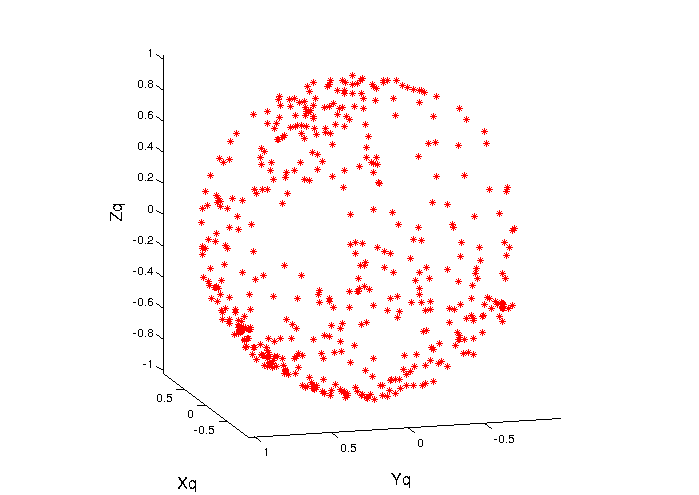
\includegraphics[width=0.5\textwidth]
		{./pics/bolacalib.png}}
	
  \end{center}
  \caption{Medias de campo magnético Terrestre}
\end{figure}

La relación que se obtiene entre la medida del sensor descalibrado y el calibrado es:
\begin{equation}
m_{calib}=U(m-c)
\end{equation}

donde 
$$
U=\left( \begin{array}{ccc}
 0.00473160006403247   &  -2.18916898319836\times10^{-5}    &  0.000309423482503981 \\
                         0      & 0.00455025410014059   &   7.83170752308679\times10^{-5} \\
                         0     &                    0   &    0.00534686558080686 \\
\end{array}
\right)
$$

$$
c=\left(\begin{array}{c}
23.3152609806586
         -126.624459617958
          19.0429011162953
\end{array}\right)
$$

Luego de calibrado el sensor se quiere determinar la capacidad que tiene el mismo de proporcionar una adecuada orientación. Con dicho fin se utiliza la tabla larga para alinear el sensor en una dirección en particular. La ubicación donde fue realizado el experimento se encuentra marcada aproximadamente con la marca roja en la figura \ref{fig:mapa}. El objeto elegido para realizar la alineación es el que se muestra en la parte superior de la figura \ref{fig:mapa}, su ubicación es la indicada por el ``muñeco'' en la figura \ref{fig:mapa}.
\begin{figure}
  \begin{center}
	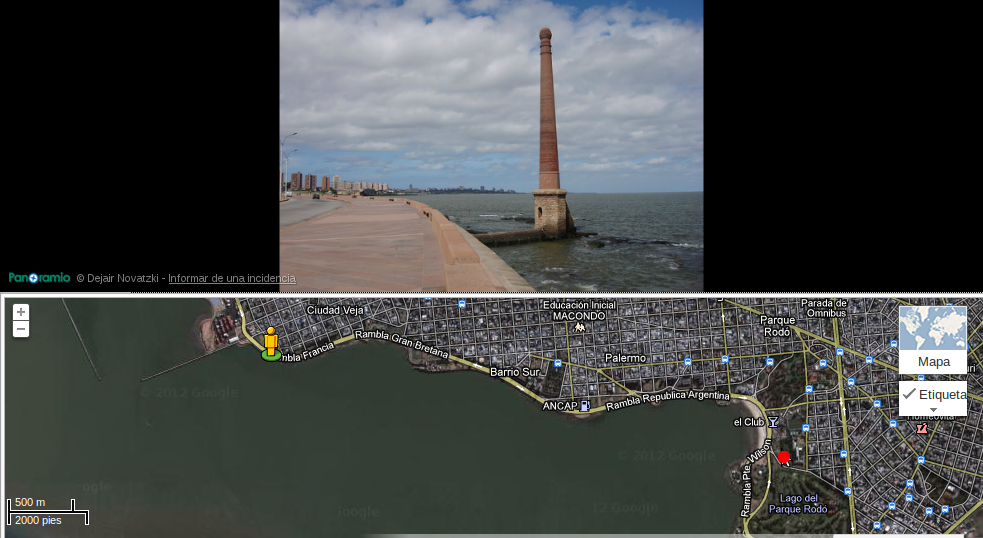
\includegraphics[width=0.8\textwidth]
		{./pics/mapa.png}
	
  \end{center}
  \caption{Mapa de la costa de Montevideo}
  \label{fig:mapa}
\end{figure}

Del mapa de la Intendencia de Montevideo \footnote{http://sig.montevideo.gub.uy/mapas/mapa-principal} se obtienen las coordenadas de los puntos seleccionados. El punto en que fue realizado el experimento es el (576039,6135625) y el punto con el cual se alineo es el (572118,6136415). El ángulo de la recta que une los dos puntos medido respecto del eje Sur-Norte es de $78.6^\circ$ al Oeste.

Se trabajó con tres \emph{sets} de orientaciones. 
\begin{itemize}
\item Orientación z. Se ubico el eje $Z_q$ (la orientación estará definida por el ángulo entre la dirección Norte y este vector) perpendicular a la superficie de la Tierra y perpendicular a la dirección definida. $X_q$ se ubica perpendicular a la superficie de la Tierra.  Luego se rotó la plataforma en sentido anti-horario 30,45,60,90,180 grados. 
\item Orientación x. En este caso el eje $-X_q$ ocupa el lugar que  tenía el eje $Z_q$. El eje que se ubica perpendicular a la superficie de la Tierra es $Y_q$. Se rotan los mismos ángulos que en el experimento anterior.
\item Orientación y. El eje $Y_q$ es el vector de orientación y el eje $-Z_q$ se ubica perpendicular a la superficie de la Tierra. 
\end{itemize} 


En la tabla \ref{tab:angulos} se presentan los resultados obtenidos para cada orientación. 



\begin{table}
\begin{tabular}{|p{50pt}|p{50pt}|p{50pt}|p{50pt}|p{51pt}|p{50pt}|p{50pt}|}
\hline
 {\cellcolor[gray]{0.6} \textbf{Rotación}}  
& \multicolumn{2}{|p{113pt}|}{\cellcolor[gray]{0.6} \textbf{Orientación z}}  
& \multicolumn{2}{|p{114pt}|}{\cellcolor[gray]{0.6} \textbf{Orientación x}}
& \multicolumn{2}{|p{113pt}|}{\cellcolor[gray]{0.6} \textbf{Orientación y}} 
\\ \hline 
   
& \multicolumn{1}{|p{50pt}|}{\cellcolor[gray]{0.7} \textbf{ángulo medido}} 
& \multicolumn{1}{|p{50pt}|}{\cellcolor[gray]{0.8} \textbf{ángulo teórico}}
& \multicolumn{1}{|p{50pt}|}{\cellcolor[gray]{0.7} \textbf{ángulo medido}} 
& \multicolumn{1}{|p{51pt}|}{\cellcolor[gray]{0.8} \textbf{ángulo teórico}}
& \multicolumn{1}{|p{50pt}|}{\cellcolor[gray]{0.7} \textbf{ángulo medido}} 
& \multicolumn{1}{|p{50pt}|}{\cellcolor[gray]{0.8} \textbf{ángulo teórico}}
\\ \hline

 0    &    -20.25  & 11.39& 162.77& 168.61&-15.33 & -11.39\\ \hline
 30   &   12.69    & 18.61& 191.38& 198.61&14.54 & 18.61 \\ \hline
 45   &   27.93 	  &	33.61 & 205.84 & 213.61 & 29.97 & 33.61 \\ \hline
 60   &   42.93 	  & 48.61 & 219.68 & 228.61 & 43.42 & 48.61 \\ \hline
 90   &   75.56 	  & 78.61 & 248.96 & 258.61 & 72.14 & 78.61 \\ \hline
 180  &   163.57	  &	168.61& 334.25 & 348.61 & 156.95 & 168.61 \\ \hline
 
\end{tabular}
\caption{Ángulos medidos y teóricos en las distintas posiciones}
\label{tab:angulos}
\end{table} 


El error promedio obtenido es $\mu=6.83^\circ$, la desviación estándar obtenida es $\sigma
=2.95^\circ$

\end{document}


